\documentclass[a4j,10pt,dvipdfmx]{jsarticle}
\usepackage[dvipdfmx]{graphicx}
\usepackage{listings,jvlisting}
\usepackage{here}

\lstset{
  basicstyle={\ttfamily},
  identifierstyle={\small},
  commentstyle={\small\itshape},
  keywordstyle={\small\bfseries},
  ndkeywordstyle={\small},
  stringstyle={\small\ttfamily},
  frame={tb},
  breaklines=true,
  columns=[l]{fullflexible},
  numbers=left,
  xrightmargin=0zw,
  xleftmargin=3zw,
  numberstyle={\scriptsize},
  stepnumber=1,
  numbersep=1zw,
  lineskip=-0.5ex
}

\begin{document}
\title{ソフトウェア設計と品質 中間課題}
\author{23B30925 横井風羽}
\date{2026/1/12}
\maketitle

\section{静的構造}

\subsection{モデリングしたクラス図}
Packmanゲームのクラス図を以下に示す。

\begin{figure}[H]
  \centering
  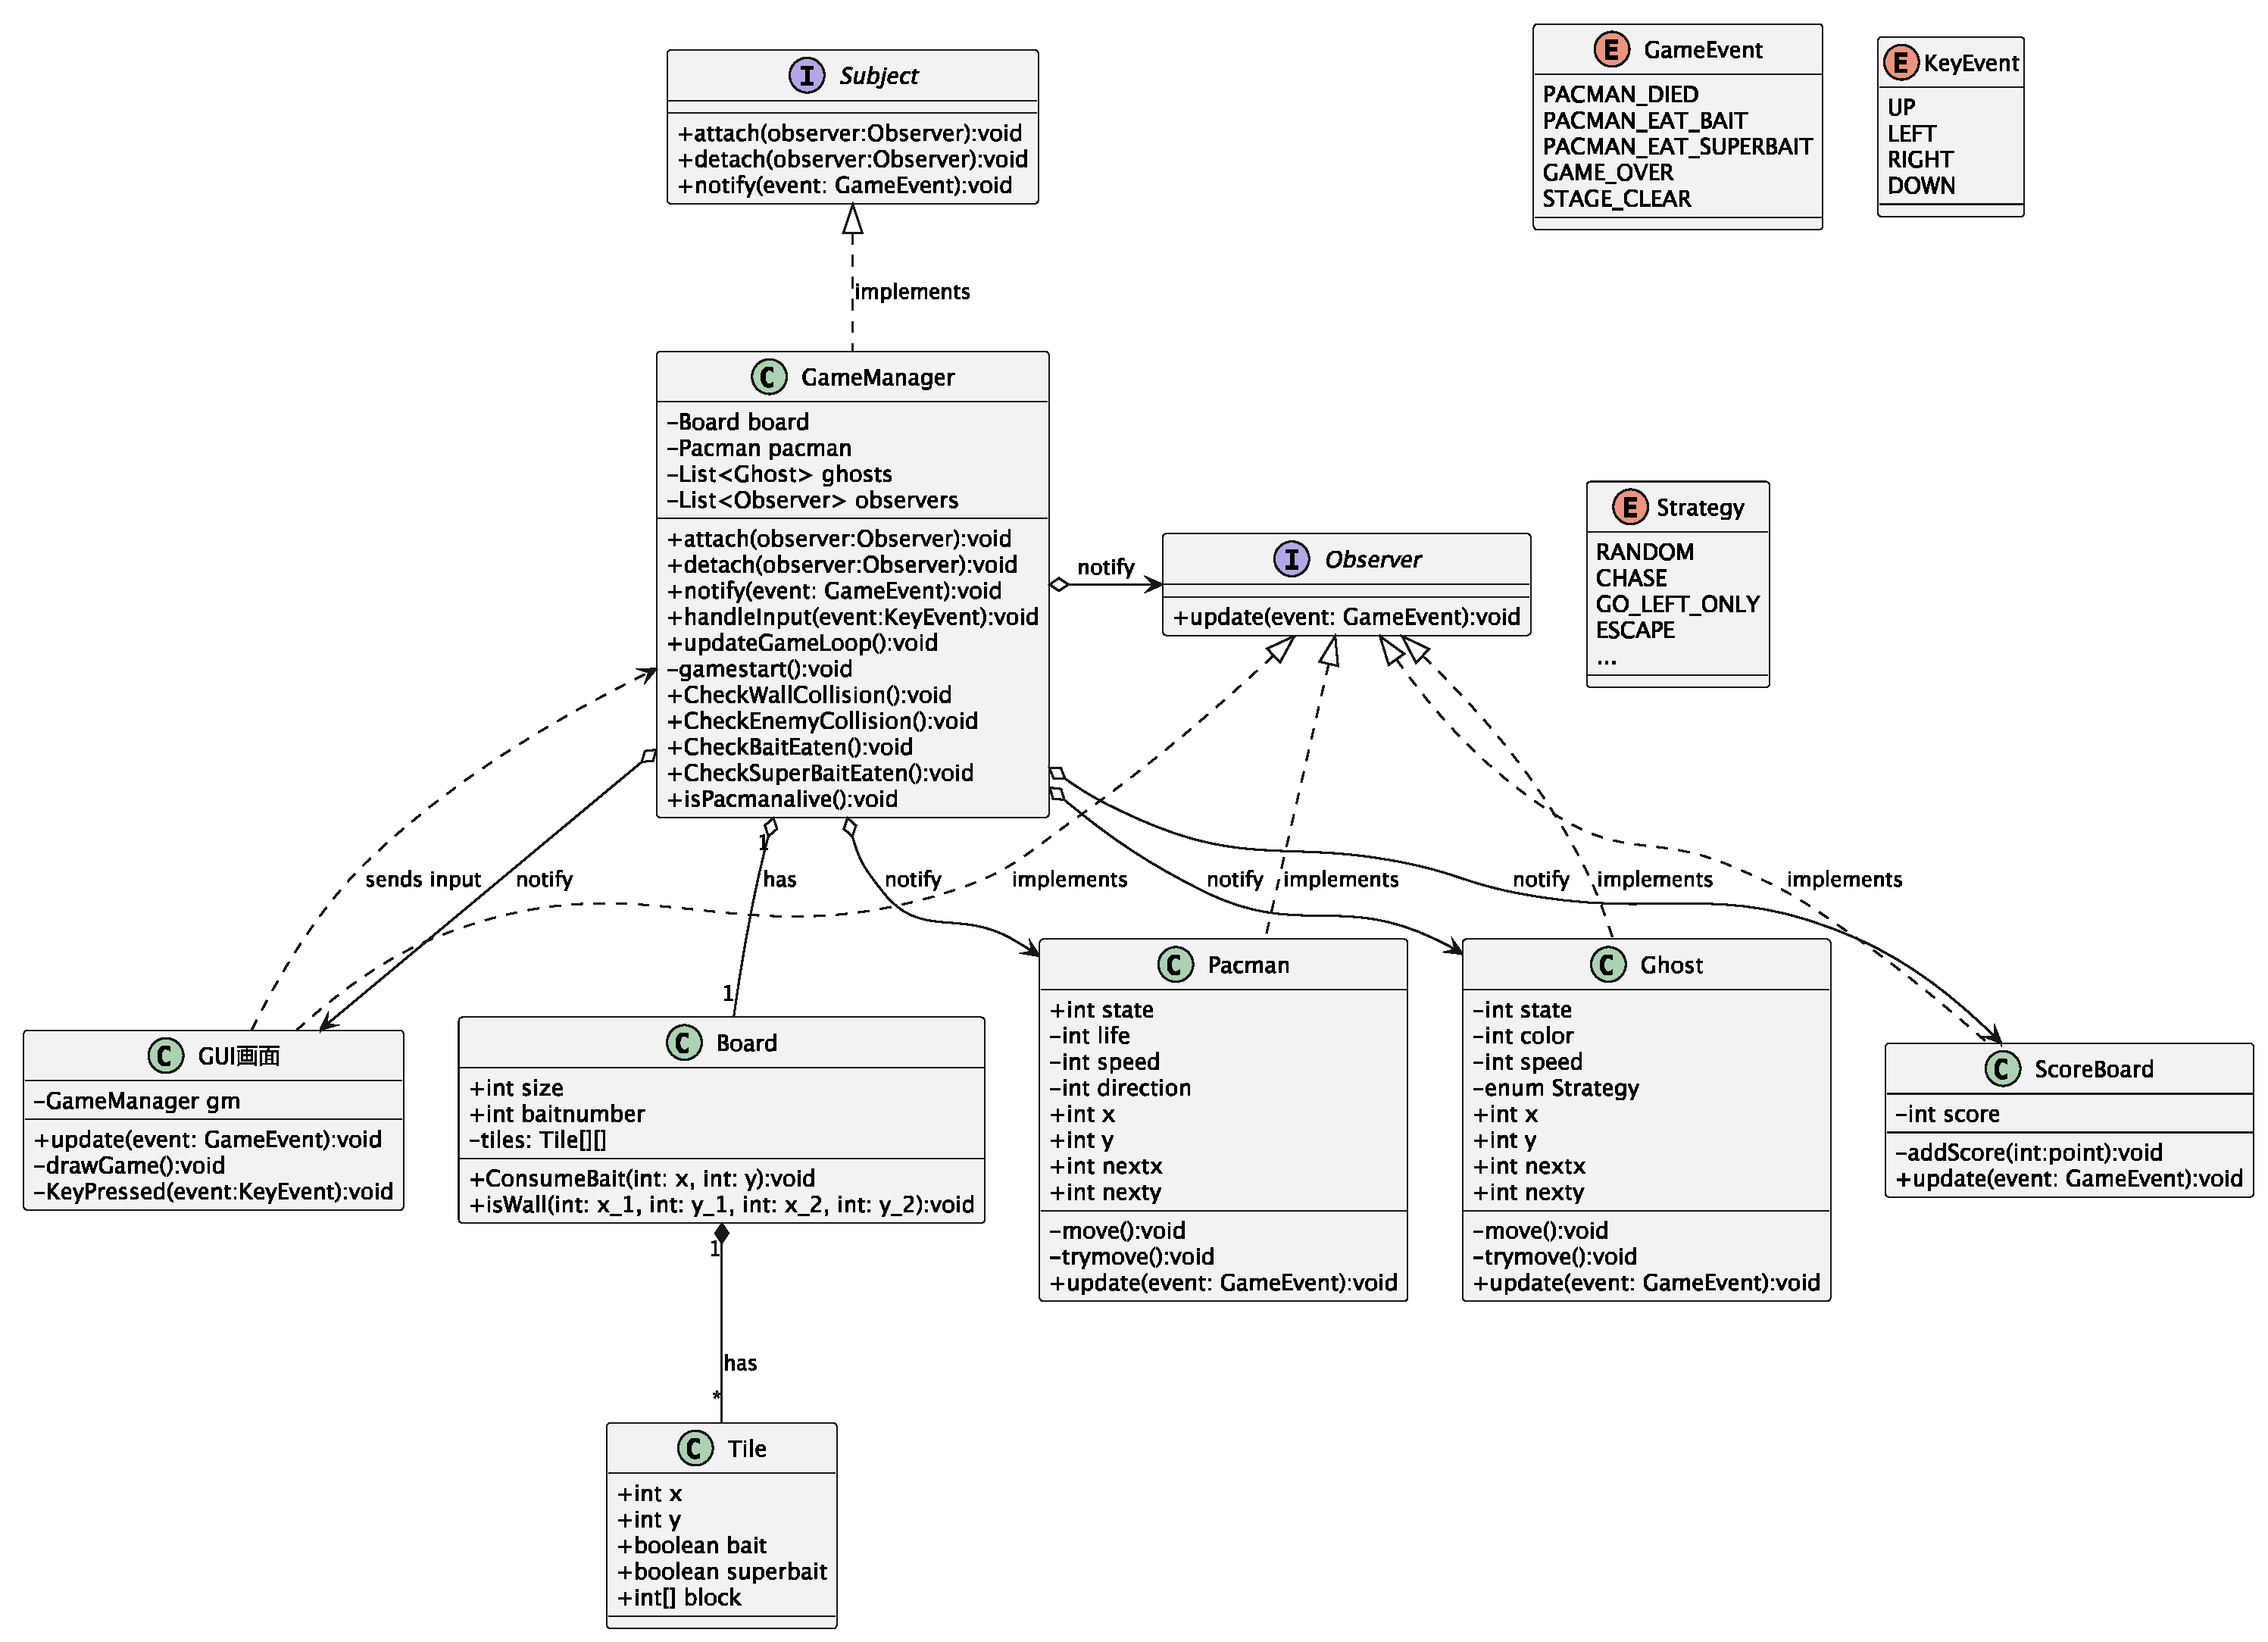
\includegraphics[width=0.95\linewidth]{class.eps}
  \caption{クラス図}
  \label{fig:class_diagram}
\end{figure}

\subsection{主要なクラスの簡単な説明}

\begin{itemize}
    \item \textbf{GameManager (GM)}: ゲーム全体の状態(パックマン、ゴースト、ボードなど)を保持し、ゲームループや入力処理、衝突判定などのロジックを統括する。Subjectインターフェースを実装し、Observerへイベントを通知する。
    \item \textbf{Pacman}: プレイヤーが操作するキャラクター。自身の位置、ライフ、速度、移動方向などを管理する。ObserverとしてGameManagerからのイベントを受け取り、状態を更新する。
    \item \textbf{Ghost}: 敵キャラクター。移動戦略(Strategyパターンを想定)に基づき自動で動作する。Pacmanと同様にObserverとして機能する。
    \item \textbf{Board}: ゲーム盤面を表す。タイルの配置、壁の判定、エサの管理を行う。
    \item \textbf{GUI画面 (Display)}: ゲームの視覚的表現を担当する。Observerとしてイベントを受け取り、画面の再描画を行う。
    \item \textbf{Subject / Observer}: Observerパターンを実現するためのインターフェース。イベント駆動型の更新通知を行う。
\end{itemize}

\subsection{全体の設計理由}
ゲームの状態変化(エサを食べた、衝突した、クリアした等)を複数のコンポーネント(画面表示、スコア、各キャラクター)に効率よく伝達するために、\textbf{Observerパターン}を採用した。これにより、\texttt{GameManager}がイベントを発行するだけで、各オブジェクトが自律的に対応する動作を行えるようになり、結合度を下げている。また、ゴーストの動きには将来的に様々なアルゴリズム(ランダム、追跡、先回り等)を適用できるよう配慮した設計としている。

\section{動的振舞いの例}

\subsection{シナリオ実行のシーケンス図}
以下のシナリオにおけるシーケンス図を示す。
\begin{enumerate}
    \item パックマンを右に移動させエサを獲得する。
    \item もう1マス右に行こうとしたら壁があって動けない。
    \item その後、モンスターがぶつかってきてライフが1つ減り、リスタートする。
\end{enumerate}

\begin{figure}[H]
  \centering
  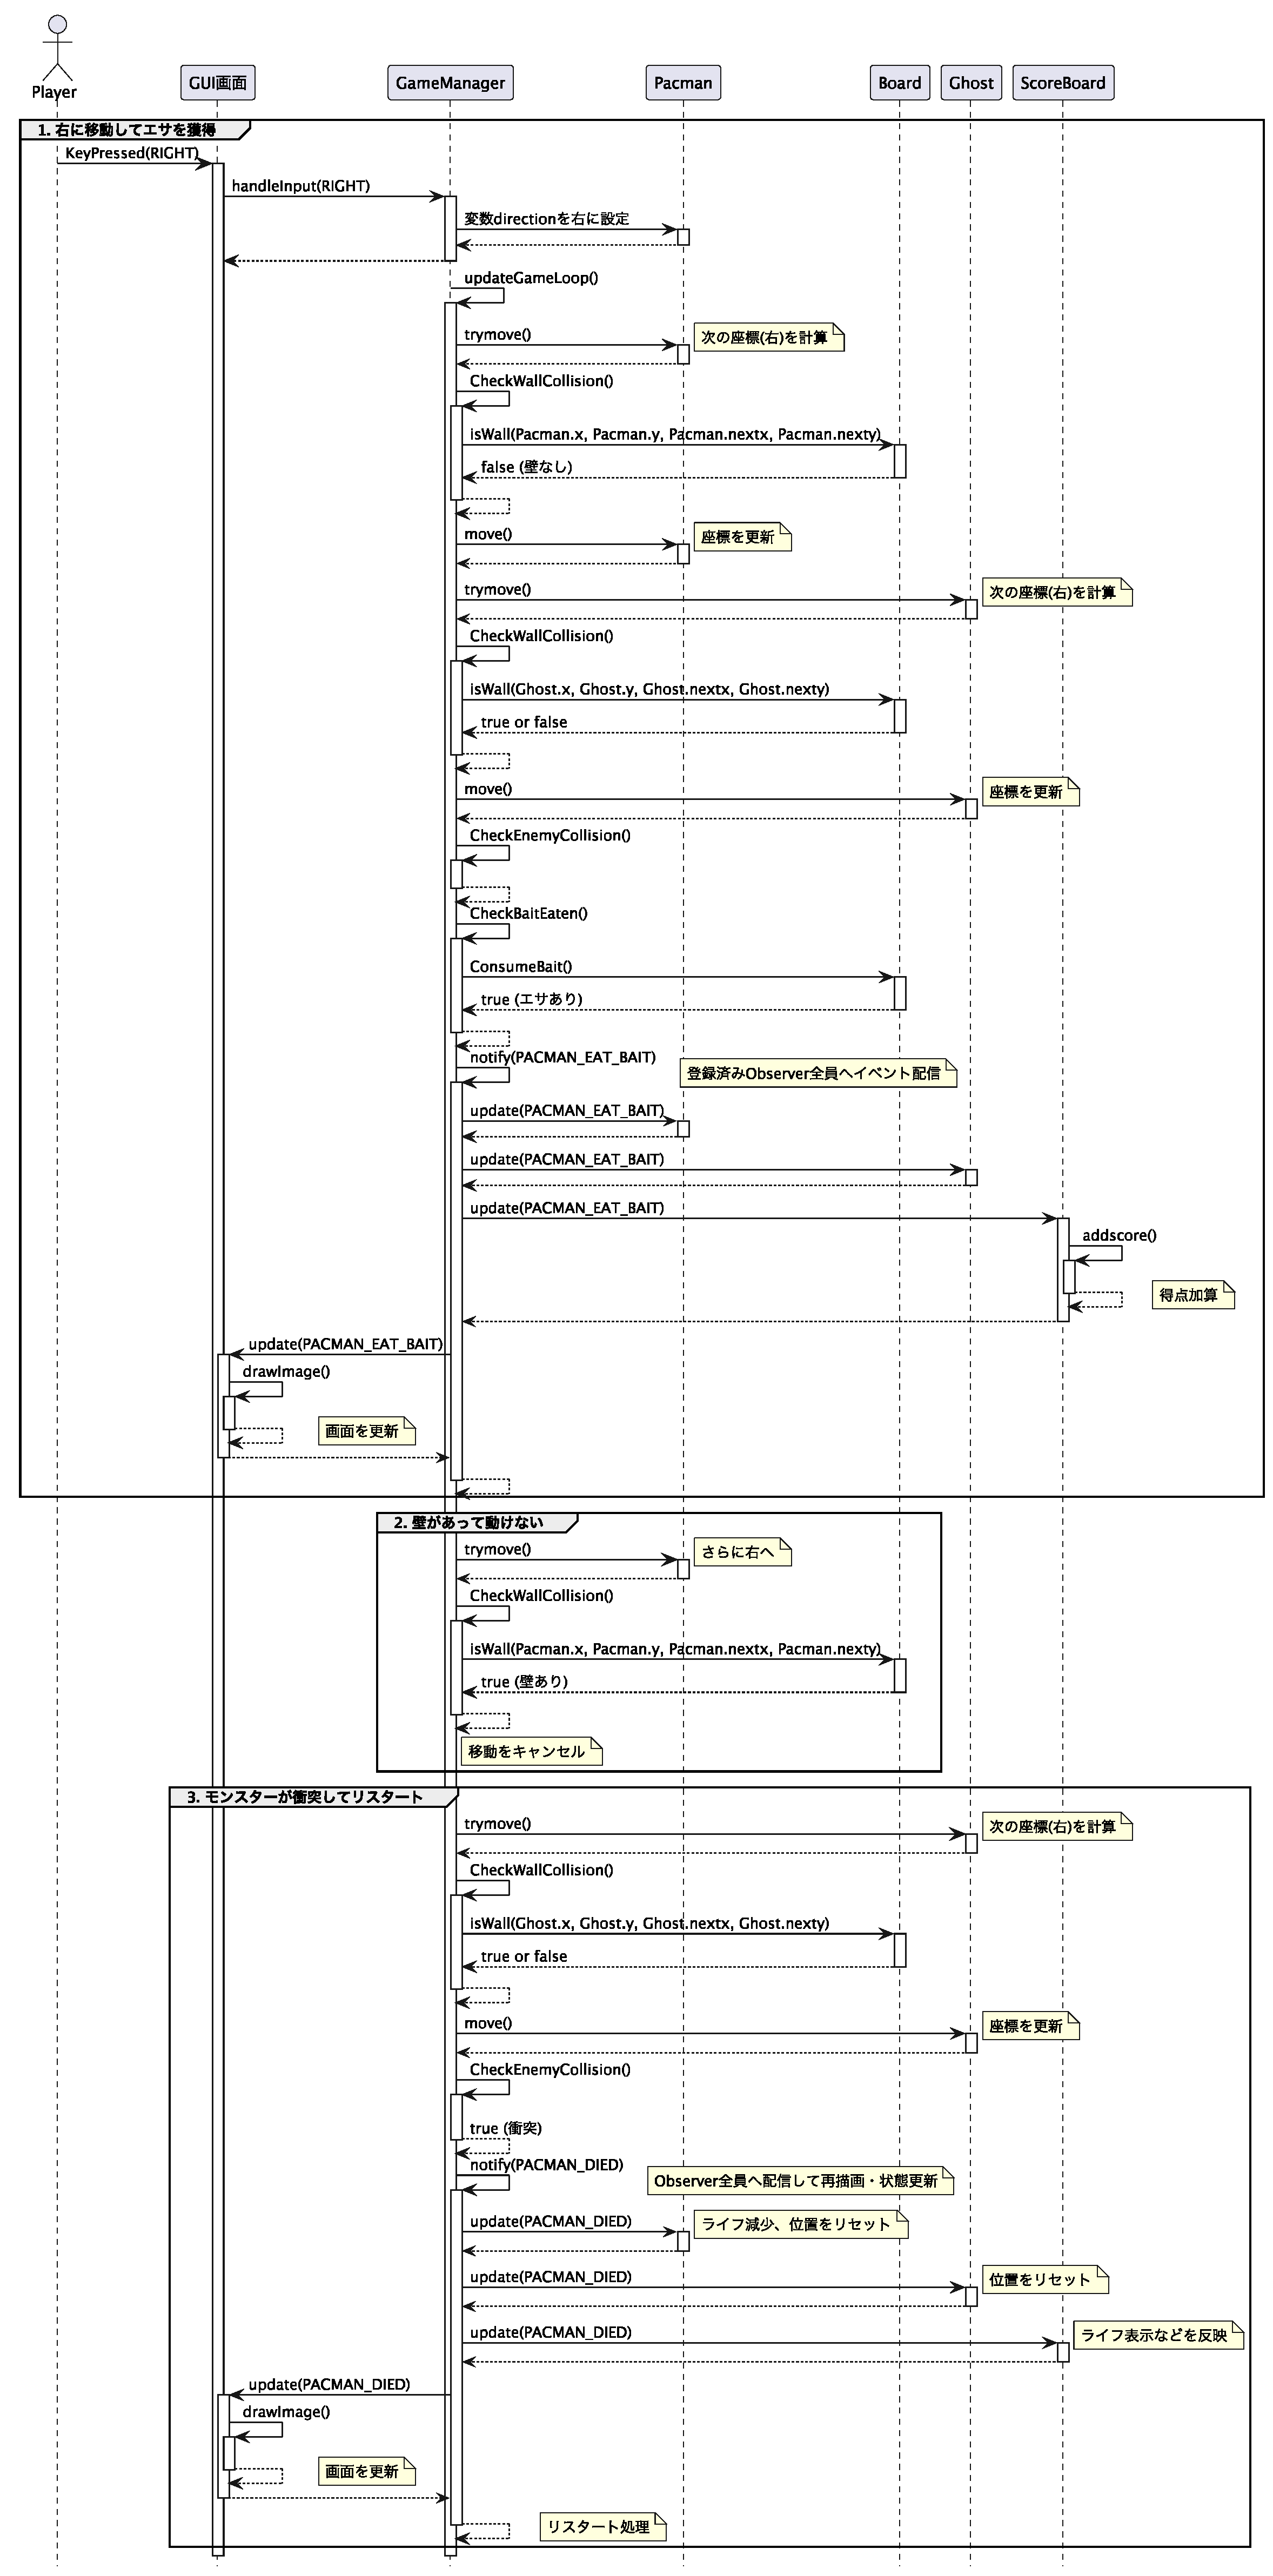
\includegraphics[width=0.7\linewidth]{sequence.eps}
  \caption{シーケンス図}
  \label{fig:sequence_diagram}
\end{figure}

このシーケンス図では、ユーザー入力 \texttt{KeyPressed} から始まり、\texttt{GameManager} が移動判定 \texttt{trymove}、壁判定 \texttt{CheckWallCollision}、イベント通知 \texttt{notify} を行う流れを表現している。特に、エサ獲得時(\texttt{PACMAN\_EAT\_BAIT})や衝突時(\texttt{PACMAN\_DIED})に、Observerパターンを通じて各インスタンスが一斉に更新される様子が確認できる。

\section{独自に想定した仮定}
なし

\section{工夫点}
\begin{itemize}
    \item \textbf{Observerパターンの活用}: ゲーム内のイベント(死亡、スコア獲得など)を一元管理し、スパゲッティコード化を防いでいる点。
    \item \textbf{責任の分離}: \texttt{Board}クラスに盤面判定ロジックを集約し、キャラクタークラスは自身の移動ロジックに集中できるようにした点。
    \item \textbf{拡張性}: ゴーストの行動パターンを\texttt{Strategy}として定義可能な構造にしており、後からの機能追加を容易にしている点。
\end{itemize}

\section{感想}
クラス図とシーケンス図を作成することで、実装前にオブジェクト間の責務分担を明確にすることの重要性を再認識した。特にObserverパターンを導入することで、イベント処理の流れが整理され、見通しの良い設計になったと感じる。PlantUMLを用いることで、修正が容易なテキストベースでのモデリングができ、試行錯誤がスムーズに行えた。

\end{document}